% LaTeX Template for writing mathematics papers.
\documentclass[reqno]{amsart}
\usepackage[all,ps,cmtip]{xy}

% Import the style file
\usepackage{algebraPaper}

% Bibliography
\usepackage[]{biblatex}   % First argument is for the bibliography style.
\bibliography{algebra.bib}

\begin{document}

% Author details.
\author{J. Borger}
\address{Mathematical Sciences Institute, Australian National University, Australia}
\email{james.borger@anu.edu.au}

\author{R. Culling}
\address{Te Kura P\={a}ngarau, Te Whare W\={a}nanga o Waitaha, Aotearoa}
\email{robert.culling@canterbury.ac.nz}

% Paper title
\title{The \'{E}tale Fundamental Group $\bn$}


\begin{abstract}
We define affine $\mathbb{N}$-schemes over the natural numbers as representable functors from the category of semirings to the category of sets. Finite \'{e}tale morphisms are defined to be those that are fppf locally totally split. For a fixed appropriately connected semiring $R$ (together with an appropriate choice of base point), the category of finite \'{e}tale morphisms is shown to be a Galois category. We conclude with the calculation of the \'{e}tale fundamental group of various semirings.
\end{abstract}

\maketitle

\tableofcontents

\section{Introduction}

In 1973 Grothendieck gave a seminar in which he \emph{defined} an affine scheme to be a representable functor from the category of (commutative unital) rings to the category of sets \cite{ega}. Betrand To\"{e}n and Michel Vaqui\'{e} presented a theory of schemes for commutative monoid objects in a symmetric monoidal category \cite{toenvaquie}. In the case the monoidal category is the category of commutative monoids, their theory describes schemes for the category of commutative unital semirings.

In this paper we follow the spirit of these authors with the following definitions. Let us denote the category of semirings $\nalg$.\footnote{Johnathon Golan's \emph{Semirings and Their Applications} \cite{golan} has most of the details we use for semirings. One can find results about the category of semirings in Borger's \cite{}. Those properties of immediate relevance will be detailed throughout the paper.} For a fixed semiring $R$ we denote the representable functor $\specr: \nalg \rightarrow \catset,$
such that $\specr(A):= \homn(R,A)$. We call such a functor an affine $\bn$-scheme and denote the category of such objects (with morphisms being natural transformations) by $\naff$. This is equivalent to $\nalg^{\text{op}}$ by the Yoneda Lemma.

With this geometric language at hand, we can ask how much of the theory of algebraic geometry can be brought over to this broader category of $\mathbb{N}$-schemes. Due to the category theoretic style of Grothendieck's development of algebraic geometry one should believe that all of the theory can be understood in the context of affine $\bn$-schemes. In this paper we explore Grothendieck's theory of the fundamental group \cite{sga1} for affine affine $\bn$-schemes. Grothendieck mentioned in Exercise 2.7.5 of [SGA IV, Expose iv, 1971] that his theory of the fundamental group will work for the category of locally constant objects of an appropriately connected topos. Peter Johnstone has the details of this work spelled out in Section 8 of Topos Theory \cite{topostheory}. We say that an affine $\bn$-scheme $X = \specr$ is connected if the only set of idempotents in $R$ with the following properties (i) $e_{i}e_{j} = \delta_{ij}e_{i}$, and (ii) $\sum_{I}e_{i} = 1$, is $\{0,1\}$. Otherwise we say $X$ is disconnected, in which case $X \cong \coprod_{N} U_{i}$ for some finite number $|N|$ of affine $\bn$-schemes $U_{i}$.

Betrand To\"{e}n and Michel Vaqui\'{e} introduced the fpqc (Grothendieck) topology to their categories of schemes in \cite{toenvaquie}. We will use this topology when we say something is happening locally. In algebraic geometry the locally constant morphisms are called finite \'{e}tale.

\begin{defn}[Finite \'{E}tale Morphism]
Let $X,Y$ be affine $\bn$-schemes and $f: Y \rightarrow X$ be a morphism of affine $\bn$-schemes. If there exists an fpqc cover $(U_{i} \rightarrow X)_{i \in I}$ of $X$ such that, for each $i \in I$ there are finite sets $N_{i}$ and isomorphisms $\varphi_{i}: Y\times_{X}U_{i} \isom \coprod_{N_{i}}U_{i}$, then we say the morphism $f:Y \rightarrow X$ is finite \'{e}tale.

If $\varphi: Y\rightarrow X$ is finite \'{e}tale and $Y \cong \coprod_{N}X$, for some finite set $N$, then we say that this finite \'{e}tale morphism is trivial.
\end{defn}

For a fixed affine $\bn$-scheme $X$ we denote the category of finite \'{e}tale morphisms over $X$ as $\fex$, where the morphisms are morphisms over $X$. This is our category (in fact, topos) of locally constant objects from which we will define the \'{e}tale fundamental group of $X$.

To define the notion of a point (fundamental functor) for our theory, we use simple semirings. We say a semiring $R$ is simple if it has precisely two congruence relations: in which case we will also refer to $X = \specr$ as a simple affine $\bn$-scheme. If a simple affine $\bn$-scheme $p$ has no non-trival finite \'{e}tale covers, then we refer to $p \rightarrow X$ as a geometric point of $X$. If $X \in \naff$, then $\spec(\overline{k}) \rightarrow X$ for separably closed fields $\overline{k}$ are examples of geometric points. An example of a geometric point not in $\zaff$ is $p = \spec(\bb)$

\begin{defn}[Geometric Morphism]
  Let $X$ be an affine $\bn$-scheme. If $p$ is a simple affine $\bn$-scheme with no non-trivial finite \'{e}tale morphisms, then we say a morphism $i: p \rightarrow X$ is a geometric morphism.
\end{defn}

For a fixed scheme $X$ and geometric point $i:p \rightarrow X$, we can define a functor $-\times_{X}p: \fex \rightarrow \catset$, by pulling back along the geometric point. Throughout the paper, we abuse this notation and use $p$ to denote both the geometric morphism and the functor above.

In this paper we show for a connected affine $\bn$-scheme $X$ the category $(\fex, p)$ (with a choice of geometric point $p$) is a Galois category. We call the the automorphism group of the fundamental functor the \'{e}tale fundamental group of $X$ and denote it $\etfg(X):= \Aut(-\times_{X}p)$. We conclude the paper by calculating this group for a number of affine $\bn$-schemes. For example we show $\etfg(\spec(\bn)) \cong 0$.

\vspace{1em}
{\bf Acknowledgments:}
Most of this work was done during Robert Culling's time as James Borger's PhD student at the Australian National University, from 2015 through 2019. This work is presented in much more detail in Culling's thesis which can be found online \cite{}. Culling would like to acknowledge the support of the Mathematical Sciences Institute at ANU and the support from the Australian People through the Australian Government Research Training Program Stipend and Scholarship. Without this kindness the work would not have been completed.

\section{Main Theorem: $\fex$ is a Galois Category}

Definition 8.4 of \emph{Topos Theory} states that a Galois category is a pair $(\mathcal{G},F)$ where $\mathcal{G}$ is a small Boolean (pre)topos and $F:\mathcal{G}\rightarrow \catset$ is an exact, isomorphism reflecting functor to the category of finite sets \cite{topostheory}.

\begin{lemma}\label{fex:BooleanTopos}
  If $X$ is a connected affine $\bn$-scheme, then $\fex$ is a Boolean (pre?)topos.
\end{lemma}

\begin{proof}


\end{proof}

\begin{lemma}\label{f:exactReflecting}
If $X$ is a connected affine $\bn$-scheme and $i:p \rightarrow X$ is a geometric point, then the functor $-\times_{X}p: \fex \rightarrow \catset$ is exact and reflects isomorphisms.
\end{lemma}

\begin{proof}


\end{proof}

\begin{thm}
If $X$ is a connected affine $\bn$-scheme $i:p \rightarrow X$, then the pair $(\fex,p)$ is a Galois category.
\end{thm}

\begin{proof}
This follows from Lemma \ref{fex:BooleanTopos} and Lemma \ref{f:exactReflecting}
\end{proof}


By the structure theorem for Galois categories we know that any two fundamental functors are (non-canonically) isomorphic, so we will often just refer to the category $\fex$ as being a Galois category.

\section{Booleans $\bb$}

For each prime $p \in \bz$ we obtain a finite field $\fp$. In the broader context of $\bn$ we find that there is only one more finite (semi-)field, the Booleans $\bb:=\{0,1\}$. All of the arithmetic is defined by the axioms of semiring, except that we force $1 + 1 = 1$.

\begin{thm}
$\etfg(\spec(\bb)) \cong 0$
\end{thm}

\begin{proof}
  Suppose the morphism of affine $\bn$-schemes $f:X\rightarrow \spec(\bb)$ is a non-empty finite \'{e}tale $\bb$-scheme --- if $X$ is empty, then $X$ is isomorphic to the empty coproduct of copies of $\spec(\bb)$. This means there exists a cover $(g_{i}:U_{i} \rightarrow \spec(\bb))_{i \in I}$ over which $f$ becomes trivial. Since the $g_{i}$ form a faithful cover, there exists $j \in I$ such that $U_{j} \neq \emptyset$. There exists a morphism $x:\spec(\bb) \rightarrow U_{j}$ --- there can be no such map from the spectrum of a field, as this would correspond to a semiring map from $\bb$ to a field, so there must be a morphism from $\spec(\bb)$

  \begin{center}
  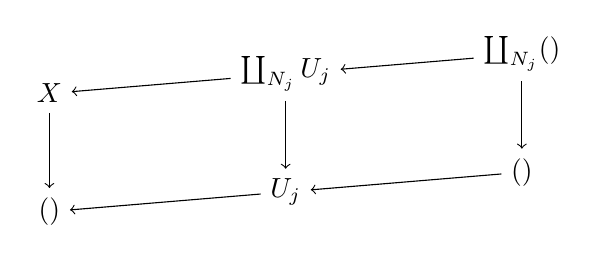
\begin{tikzpicture}
  \node (A) at (0,1) {$\coprod_{N_{j}}U_{j}$};
  \node (B) at (0,-0.5) {$U_{j}$};
  \node (C) at (3,-0.25) {$\spec(\bb)$};
  \node (D) at (3,1.25) {$\coprod_{N_{j}} \spec(\bb)$};
  \node (E) at (-3,-0.75){$\spec(\bb)$};
  \node (F) at (-3,0.75){$X$};
  \path[->]
  (F) edge (E)
  (B) edge (E)
  (A) edge (F)
  (D) edge (A)
  (C) edge (B)
  (A) edge (B)
  (D) edge (C)
  ;
  \end{tikzpicture}
  \end{center}

  The composition along the bottom (the identity) is an isomorphism, therefore the top row must also be an isomorphism. It follows that $X \cong \coprod_{N_{j}} \spec(\bb)$; that is to say, $X$ is totally split. Therefore all affine $\bn$-schemes that are finite \'{e}tale over $\spec(\bb)$ are totally split.
\end{proof}

\section{Non-negative Real Numbers $\br_{+}$}

\begin{thm}
$\etfg(\spec(\br)) \cong 0$
\end{thm}

\begin{proof}

As for all of the previous calculations, we need only show that every finite \'{e}tale morphism over $\br_{+}$ is trivial. For this proof we use the Galois theory of $\bc$ and the above result about the Galois theory of $\bb$ to compare the fiber of a finite \'{e}tale morphism $\br_{+} \rightarrow A$ over $\bc$ and $\bb$. This comparison yields the theorem.

\begin{center}
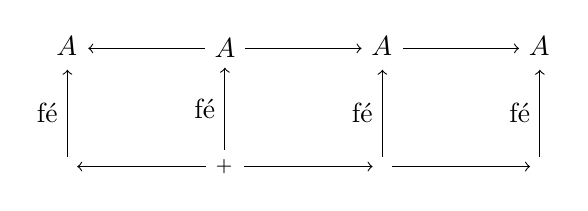
\begin{tikzpicture}
\node (C) at (-2,1.5) {$A_{\bb}$};
\node (D) at (0,1.5) {$A$};
\node (I) at (2,1.5) {$A_{\br}$};
\node (I') at (4, 1.5) {$A_{\bc}$};
\node (A) at (0,0) {$\br_{+}$};
\node (B) at (-2,0) {$\bb$};
\node (J) at (2,0) {$\br$};
\node (J') at (4,0) {$\bc$};
\path[->]
(A) edge node[left] {f\'{e}}  (D)
(A) edge (B)
(B) edge node[left] {f\'{e}} (C)
(D) edge (C)
(J) edge node[left] {f\'{e}} (I)
(J) edge (J')
(J') edge node[left] {f\'{e}} (I')
(I) edge (I')
(A) edge (J)
(D) edge (I)
;
\end{tikzpicture}
\end{center}
\end{proof}


\section{Natural Numbers $\bn$}

\begin{thm}
$\etfg(\bn) \cong 0$
\end{thm}

\section{Non-negative Sub-algebras of Real Number Fields}

\section{Tropicl Real Numbers $\bt$}

People will ask...

\newpage
\printbibliography
\vspace{2em}
\end{document}
